\section{Реализация}
\label{sec:implementation}

В этом разделе наше внимание сместится на осбенности реализации процессов
связанных с типами в Scala Plugin и особенности их инструментирования.
\textbf{Так как конечной целью является визуализация работы этих процессов, то
хочется максимально опираться на стандарт языка, которым является спецификация
scala \cite{scala_spec}.}
Мы проследим как соответсвующие понятия из спецификации переносятся в Scala Plugin.
А там где это не возможно будет явно указано на расхождение в реализации плагина и
спецификации.
Так-же будет указано как визуализируется каждый процесс.

% Реализация в плагине в плагине
% Смысл в последующей визуализации
% Хочется сделать С уважением к спецификации
% Однако не везде это возможно сделать
% Где можно сделаем
% Везде будет указано расхождение

До этого момента, когда мы говорили о работе плагина, то использовали
нейтральное слово процесс.
Теперь нужно вспомнить, что изначальной задачей было явно визуализировать
работу связанную с типами, которую плагин делает неявно.
Архитектура части плагина связанной с типами будет
рассмотрена в разделе \ref{sec:arch}.
Перечислим интересующие нас процессы.

Базовым процессом является сравнение двух типов.
В спецификации для этого вводятся три понятия: эквивалентность типов, сводимость
типов и слабая сводимость типов.
Эквивалентность означает что один тип мы в любом контексте можем заменить другим
типом, и это отношение наиболее понятно интуитивно.
Сводимость типов намного более интересна и используется во всех других процессах.
Ее мы рассмотрим в разделе~\ref{sec:conformance}.
Там же будет описание слабой сводимости, а также будет разобрано представление
типов в Scala Plugin и их отличия от типов описанных в спецификации scala.

Следующим интересующим нас процессом будет вывод типов.
Важно что вывод типов в плагине и в спецификации осуществляется по разному.
Подробно об этом будет написано в разделе~\ref{sec:infer}

Последний процесс, следующий из вывода типов - это разрешение перегрузок функций.
Действительно, типовые переменные появляются в вызовах полиморфных
функций и их неявный вывод актуален для конкретного вызова.
А так как в scala присутствуют перегрузки функций, то прежде всего нужно
разрешить символ на котором были вызваны аргументы.
Процесс разрешения перегрузок будет рассмотрен в разделе~\ref{sec:overloading}.

Отдельного упоминания заслуживает механизм implicit.
В данной работе не затрагивались неявные преобразования и неявные параметры.
В рамках Scala Plugin уже существуют ShowImplicitParametersAction, показывающий
неявно передаваемые параметры, и GoToImplicitConversationAction, помогающий
в работе с неявными преобразованиями.
Так же в данной работе не освященна работа с динамическими типами.
\textbf{Еще не уделялось внимания наследованию.}

\subsection{Архитектура Scala Plugin}
\label{sec:arch}

\begin{figure}[t]
\centering
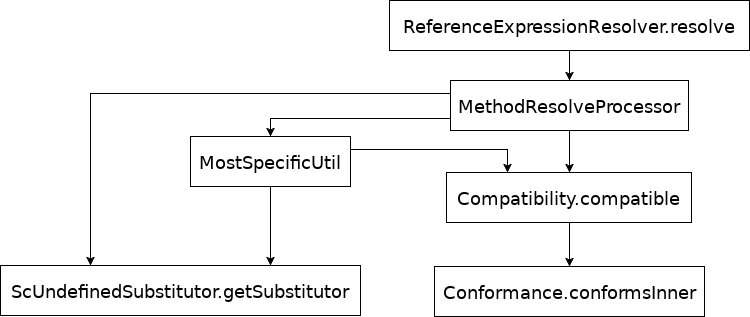
\includegraphics[width=\textwidth]{img/call-graph}
\caption{Граф вызовов}
\label{fig:callGraph}
\end{figure}

Как говорилось в начале главы~\ref{sec:implementation}, нас будут интересовать
процессы сведения типов, выведения типов и выбора перегрузки функции.
Все эти процессы можно проилюстрировать на вызове полиморфной функции.
Для начала рассмотрим как он будет обрабатываться плагином с
точки зрения архитектуры.
На рисунке~\ref{fig:callGraph}, несколько упрощенно, показан граф вызовов
такой обработки.
Мы явно будем указывать классы, основные и вспомогательные функции в которых
использовалась аннотация uninstrumented.
Это нужно чтобы понять куда именно добавлялась инструментация.
% основываясь на интересующих нас процессах

\textbf{Улучшить введение.}
Представим что у нас есть символ \textbf{f} и аргументы
\textbf{e1} ,..., \textbf{en}.
Для проверки этого применения будет вызван метод \textbf{resolve} объекта
\textbf{ReferenceExpressionResolver}.
Это и будет точкой входа.
Аннотировано uninstrumented:
\begin{itemize}
  \item \textbf{ReferenceExpressionResolver.resolve}
\end{itemize}
% Здесь только к методу \textbf{resolve} будет добавлена аннотация uninstrumented.

Далее с помощью класса \textbf{MethodResolveProcessor} будет осуществлен
поиск кандидатов обладающих таким же именем как \textbf{f}.
\textbf{MethodResolveProcessor} будет хранить множество кандидатов и
результаты применения соответсвующих кандидатов к аргументам.
Также там находится часть логики по фильтрации кандидатов, более подробно о которой
будет написано в разделе~\ref{sec:overloading}.
Аннотировано uninstrumented:
\begin{itemize}
  \item класс \textbf{MethodResolveProcessor}
  \item \textbf{MethodResolveProcessor.problemsFor}
  \item \textbf{MethodResolveProcessor.candidates}
\end{itemize}
% Аннотация uninstrumented была добавлена к самому классу
% \textbf{MethodResolveProcessor}, а также к вспомогательным методам
% объекта-компаньона \textbf{problemsFor} и \textbf{candidates}.

Для каждого кандидата нужно проверить, возможно ли вызвать его с такими аргументами.
Инструменты для этого находятся в классе \textbf{Compatibility}.
Омновная часть кода здесь - это перебор разных конструкций Scala Plugin,
описывающих исходный код, а также способов применения к ним аргументов.
Например, разбор таких случаев как передача аргумента по имени или параметры со
значением по умолчанию.
Аннотировано uninstrumented:
\begin{itemize}
  \item \textbf{Compatibility.checkConformance}
  \item \textbf{Compatibility.checkConformanceExt}
  \item \textbf{Compatibility.compatible}
\end{itemize}
% Здесь аннотация uninstrumented добавлена к методам объекта
% \textbf{checkConformance}, \textbf{checkConformanceExt} и \textbf{compatible}.

Для проверки двух типов используется интерфейс \textbf{Conformance}.
У этого интерфейса две реализации: одна для системы типов scala, другая для
системы типов dotty \cite{dotty}, нового поколения языка scala.
В обоих случаях метод \textbf{conformsInner} возвращает пару: возможна ли
сходимость и набор ограничений на абстрактные типы при которых сходимость
возможна.
Про процесс сходимости написано в разделе~\ref{sec:conformance}.
Аннотировано uninstrumented:
\begin{itemize}
  \item \textbf{Conformance.conformsInner}
  \item \textbf{Conformance.computable}
  \item \textbf{Conformance.checkParameterizedTypes}
  \item \textbf{Conformance.addParam}
  \item \textbf{Conformance.addArgedBound}
  \item класс \textbf{Conformance.LeftConformanceVisitor}
\end{itemize}
% Здесь аннотации uninstrumented применяются к методам
% \textbf{conformsInner}, \textbf{computable}, \textbf{checkParameterizedTypes},
% \textbf{addParam}, \textbf{addArgedBound}, а также к
% классу \textbf{LeftConformanceVisitor}.

Далее необходимо проверить что ограничения полученные на предыдущем шаге
возможно разрешить.
Для этого есть интерфейс \textbf{ScUndefinedSubstitutor}.
Его реализуют \textbf{ScUndefinedSubstitutorImpl} и
\textbf{ScMultiUndefinedSubstitutor}.
Отличие одной реализации от другой состоит в том, что
\textbf{ScUndefinedSubstitutorImpl} хранит только один набор ограничений, в
то время как \textbf{ScMultiUndefinedSubstitutor} хранит сразу несколько.
Это может понадобится если существует более одного способа добиться сводимости
типов. Конкретно это используется для составных типов.
Заметим, что разрешение ограничений на абстрактные типы - это и есть вывод типов.
Больше информации можно получить в разделе~\ref{sec:infer} о выводе типов.
Аннотировано uninstrumented:
\begin{itemize}
  \item \textbf{ScUndefinedSubstitutor.addLower}
  \item \textbf{ScUndefinedSubstitutor.addUpper}
  \item \textbf{ScUndefinedSubstitutor.getSubstitutorWithBounds}
  \item \textbf{ScUndefinedSubstitutor.getSubstitutor}
\end{itemize}
% Аннотация uninstrumented используется методах \textbf{addLower},
% \textbf{addUpper}, \textbf{getSubstitutorWithBounds}, а также \textbf{getSubstitutor}.

Интересно заметить, что пара \textbf{Compatibility} и
\textbf{ScUndefinedSubstitutor} образуют что-то вроде алгоритма
Хиндли-Милнера \cite{hindley–milner}.

Остался класс \textbf{MostSpecificUtil}.
Он нужен если после всех проверок сделанных \textbf{MethodResolveProcessor}
осталось больше одного кандитата.
В таком случае требуется найти наиболее специфичного кандитата.
Именно этим \textbf{MostSpecificUtil} и занимается.
Подробнее в разделе~\ref{sec:overloading}.
Аннотировано uninstrumented:
\begin{itemize}
  \item класс \textbf{MostSpecificUtil}.
\end{itemize}
% С помощью uninstrumented аннотируется только сам класс
% \textbf{MostSpecificUtil}.

% Все это было инструментровано для сбора дополнительных данных.
Всего в проекте потребовалось использовать 28 аннотаций uninstrumented.
Стоит заметить что граф вызовов сильно упрощен для улучшения понимания.
На самом деле по разным причинам все вызывают почти всех.

% Повсюду куча сравнений...\textbf{MethodResolveProcessor} \textbf{Compatibility}


\subsection{Проверка сводимости типов}
\label{sec:conformance}

В этом разделе будет рассмотрен процесс сводимости типов, будут описаны
структуры отвечающие за типы в Scala Plugin, а также дано стравнение типов
Scala Plugin и типов описанных в спецификации scala.

В спецификации scala сводимость вводится как транзитивное замыкание над
набором аксиом и правил вывода.
Это достаточно формальное определение.
Если следовать ему, то любое сведенение типов является некоторым доказательством.
А чтобы убедить кого-то в этом сведении, нужно предоставить корректное дерево
вывода.
Так что алгоритм, который занимается проверкой сводимости двух типов - это
в некотором роде система автоматического доказательства.
Существет множество систем автоматического доказательства \cite{automata},
однако наша логика слишком проста чтобы использовать, например, coq.
Так же стоит отметить, что слабая сводимость - это просто расширение набора
правил вывода для типов наследующихся от AnyVal.

В Scala Plugin для проверки сводимости на вход подаются два типа,
далее мы будем называть их левым и правым, задача свести правый к левому.
После этого для левого типа запускается шаблон посетитель, во время которого
тип конкретизируется, а после происходят проверки основанные на правилах
вывода.
Во время этих проверок посетитель может запускаться еще и для правого типа.
В самом конце идет проверка, является ли правый тип наследником левого.
Подробнее это можно посмотреть в объекте \textbf{Conformance}.

Стоит отметить что с одной стороны такой подход достаточно прост для анализа.
Однако с другой стороны в нем много избыточности, например, постоянные повторяения
одной и той логики для правого и левого типов.
Так же присутствуют постоянные проверки типов на Any и Nothing.
В первый раз они встречаются на самом верхнем уровне, а после проверки на них
присутствуют в самых неожиданных местах.
В коде можно встретить \textbf{java.lang.Object}, хотя упоминания о
нем в системе типов scala кажется странным.
Забегая вперед, одним из типов в Scala Plugin является JavaArray.
В scala для абстракции над массивом существует класс \textbf{scala.Array} и на
уровне типов это сводится к частному случаю параметризованного класса.
Отдельная сущность для массива влечет дублирование кода для параметризованных
типов, в котором и так очень много повторений.
\textbf{про несоовтетсвие типов.}
Все это сильно повышает неоднородность кода.

Теперь поговорим про визуализацию сводимости типов.
Как говорилось в начале главы~\ref{sec:implementation} сведение типов является
базовым процессом, который встречается постоянно и его наглядная визуализация
очень важна.
В качестве представления дерева мы будем использовать вложенные вкладки,
которые имеют древовоидную структуру.
Это достаточно естественное решение, учитывая что само сведение является
деревом вывода.

Узлы дерева будут делиться на два типа:
\begin{itemize}
  \item Узлы отношения.
  В этих узлах записано что рассматриваемые в данный момент
  типы должны состоять в каком-то отношении.
  Это может быть либо правда, либо нет.
  Как пример, можно рассмотреть код~\ref{lst:conformance}.
  В нем мы объявляем отношение сводимости. Оно определено для двух типов:
  правого и левого.
  Для того чтобы оно было истинным, должно быть выполнено хотя бы одно из
  условий сводимости.
  \item Узлы условий.
  Эти узлы символизируют собой аксиомы и правила вывода введенные в спецификации
  scala.
  Часть условий может иметь сложную структуру и требовать выполнения каких-то
  отношений, из-за чего структура получается рекурсивной.
  В коде~\ref{lst:condition} находится интерфейс условия для сводимости.
\end{itemize}


\begin{lstlisting}[caption={Узел условия},label={lst:condition}]
sealed trait CCondition {
  def satisfy(ctx: RelationContext): Boolean
}
\end{lstlisting}

\begin{lstlisting}[caption={Узел отношения},label={lst:conformance}]
case class Conformance(left: ScType, right: ScType,
           conditions: Seq[CCondition]) extends Relation {
  override def satisfy(ctx: RelationContext): Boolean =
    conditions.exists(_.satisfy(ctx))
}
\end{lstlisting}

Все по заповедям раздела~\ref{sec:data}.

В обоих случаях передается контекст.

В ходе работы собираются условия.
После рекурсивных вызовов полученные условия объединяются в отношения.
После этого мы получаем уже готовую для визуализации структуру.

\textbf{Картинка во вложении.}

На этом заканчивается часть про сведение типов в общем и начинается часть про
сводимость для конкретных типов.
Это позволит лучше понять отличия типов представленных внутри Scala Compiler
и спецификацией scala.
\textbf{чтобы понять типы в спецификации, лучше всего посмотреть спецификацию,
особенности синтаксиса}

% Value Types
%
% Non-Value Types

\subsubsection{Singleton Type}
Scala очень сильно использует концепцию пространств имен.
Причем не только для пакетов или типов.
В scala также у каждой переменной есть свое пространство имен.
За счет этого механизма в scala существует некоторая разновидность зависимых
типов \cite{dependent_type}, а апогеем этой идеи является DOT calculus
\cite{dot_calculus}.

Singleton type используется для того чтобы солаться на тип объекта, пакета или
переменной.
Обычно singleton type встречается когда мы хотим сослаться на тип объекта.

% правило вывода Singleton продолбано
В плагине этот тип не преставлен классом, а его роль как правило выполняет
\textbf{ScDesignatorType}.
Хоть в спецификации singleton type и вводится через концепцию пути,
\textbf{ScDesignatorType} по сути представляет оберку над ссылкой на место в коде,
где соответсвующий объект вводится.
А проверка сводимости заменяется на проверку эквивалентности.

Отдельным случаем в плагине является использование singleton type для ссылки
\textbf{this}.
В таком случае нельзя использовать просто ссылку на место в коде.
Нужно учитывать контекст в котором \textbf{this.type} встречается.
Для этого в плагине есть класс \textbf{ThisType} логика обработки которого
сводится к транзитивности и эквивалентности.


\subsubsection{Type Projection}

Любой тип в scala, согласно спецификации, лежит в каком-то пространстве имен.
И сам тип тоже образует пространство имен.
Чтобы получить доступ к типам в пространстве имен типа, используются
type projection.
\textbf{Все классы описываемые пользователем типы, а также стандартные будут такими.}
Так, например, тип представляющий целые числа будет выглядеть как
scala.type\#Int.
Здесь мы взяли базовый пакет scala, получли его singleton type, а после
спроецировали в projection type.

В Scala Plugin есть класс \textbf{ScProjectionType}, который содержит
проецируемый тип и имя проекции.
Работу с ним легко привязать к правилам сведения для type projection,
тут нет особых сложностей.

\subsubsection{Type Designator}
Для того чтобы не писать все время scala.type\#Int как в предыдущем пукте,
существуют типы являющиеся короткими синонимами для type projection.
Таким образом Int будет просто сокращением для scala.type\#Int.

Вышеупомянутый \textbf{ScDesignatorType} берет на себя и эту роль.
Правда его связь с type projections теряется, остаются проверки эквивалентности
и наследования.
Так же есть тонкость с объявлением типов, но про это будет написано в разделе
Abstract Types.

\subsubsection{Parameterized Type}
Parameterized type появляется когда у нас есть конструктор типа и мы хотим
построить применить его для конкретных типов.
Например, \textbf{List[Int]} - это parameterized type,
где \textbf{List} - это конструктор типа, принимающий один типовой
аргумент.

В плагине есть соответствующий класс \textbf{ParameterizedType}.
При работе с ним появляются понятия вариантности типовых параметров.
Логика работы с ним хоть и тяжеловесна, но повторяет правила сведения для
parameterized type.

\subsubsection{Compound Type}
Идейно, можно представлять что тип \textbf{A with B} является наибольшим
общим предком для типов \textbf{A} и \textbf{B}.
Аналогично для большего количества типов.
С другой стороны существуют структурные типы, определяющиеся набором объявлений
перменных типов и функций.
\textbf{больше про структурные типы.}
Если объединить эти две концепции, то получится compound type.

В Scala Plugin compound type представлен классом \textbf{ScCompoundType}.
Правила работы с ним соответсвуют описанным в спецификации правилам сведения.
Интересный момент возникает для ограничений на абстрактные типы.
Например, если мы пытаемся свести тип \textbf{A with B} к типу \textbf{C},
то для этого либо \textbf{A} должен сводиться к \textbf{C}, либо \textbf{B}
должен сводиться к \textbf{C}.
Нас устроит любой из вариантов, однако могут возникнуть разные ограничения на
типы.
Так как ограничения разрешаются в самом конце, то необходимо сохранить все
варианты ограничений.
Именно для этой ситуации и существет класс \textbf{ScMultiUndefinedSubstitutor},
встреченный в разделе~\ref{sec:arch}.

\subsubsection{Existential Type}
Existential type - это просто экзестенциальный тип, подробнее о котором можно
почитать в \cite{type_theory}.
Он нужен чтобы замкнуть свободные типовые переменные.
Примером такого типа будет \textbf{List[(A, A)] forSome \{ type A \}}.
Здесь мы объявили список пар, где типы первого и второго элемента пары совпадают.

В Scala Plugin для existential type используется класс
\textbf{ScExistentialType}.
Он так же как и \textbf{ParameterizedType} добавляет к типу набор переменных,
только тут эти переменные должны быть абстрактными.
Класс представляющий абстрактную типовую переменную в existential type
называется \textbf{ScExistentialArgument}.
В нем сожержится информация об имени и границах типа, а также типовых агрументах.
Последнее нужно для поддержки типов высших кайндов.
Интересный момент возникает при сведении какого-нибудь типа к existential type.
В таком случае требуется не просто найти ограничения для типовых параметров,
нужно проверить что они разрешимы, а все условия на границы типов соблюдены.
Поэтому тут решение системы ограничений на типы происходит прямо во время сведения.

\subsubsection{Method Type}

Как известно, в scala функции являются объектами первого порядка.
Иначе говоря, мы можем передавать функции как аргументы, сохранять переменные
и так далее.
Однако, мы не всегда можем выразить различные типы методов, доступные в scala,
через классы с дженериками.
Поэтому для описания методов вводится отдельный тип, называемый method type.
Этот тип нельзя выразить в синтаксисе scala, а при необходимости привести
method type к типу функции, выполняется эта-расширение~\cite{eta_expansion}.

В плагине используется для этого используется класс \textbf{ScMethodType}.
Так как method type можно свести только к method type, а его обработка
локализована и в точности повторяет то что написано в спецификации.

\subsubsection{Polymorphic Method Type}
Что бы представить в типы зависящие от типов, такие как полиморфные методы,
используется polymorphic method type.
Таким образом это он является типом, принимающим типовые аргументы,
и возвращающим некоторый внутрениий тип с подставленными аргументами.
Его так же как и method type нельзя выразить синтаксически.

В Scala Plugin его представляет \textbf{ScTypePolymorphicType}, который содержит
внутренний тип и набор типовых параметров.
Работа с ним повторяет правила вывод из спецификации.

\subsubsection{Type Constructors}
Отдельным случаем в спецификации scala рассматриваются типовые конструкторы.
В этом случае применение типовых аргументов приводит к типу который можно
инстанцировать.

В Scala Plugin его роль выполняет все тот же \textbf{ScTypePolymorphicType}.

\subsubsection{Abstract Type}

Abstract type не вводится среди основных типов в спецификации, однако упоминается
в самом начале соответсвующего раздела.
Он определяется как тип описываемый типовым параметром или объявление типа без
конкретного значения.
При работе с ним используются его верхняя и нижняя границы.

В Scala Plugin под этот случай можно подвести много классов.
В первую очередь это \textbf{TypeParameterType} который используется как тип
типового параметра.
Аналогичные правила применяются для встреченного ранее
\textbf{ScExistentialArgument}.
И сюда же попадает \textbf{ScDesignatorType}.
Как говорилось ранее, он ссылается на куски кода.
При объявления типов без конкрентных значений используется он же.

\subsubsection{Типы представленные только в спецификации scala}
Так же в scala спецификации вводятся такие типы как annotated type и infix type,
но первый не важен в рассматриваемых нами процессах, а второй является просто
синтаксическим сахаром.

Еще есть tuple type и function type.
Первый является удобной формой записи для кортежа, а второй для функции.
Оба этих типа являются синтаксическим сахаром и сводятся к параметризованным
типам в scala.
\textbf{Я не уверен что это правда для dotty!}
В плагине нет типов соответсвующих им, вместо этого он сразу производит
удаление синтаксического сахара.
Подробнее про это можно прочитать в работе \cite{kozlov}.

\subsubsection{Типы представленные только в Scala Plugin}
Хоть в Scala Plugin и отсутсвуют и отсутсвуют такие сущности как tuple type или
function type, зато он привносит свои понятия в систему типов.

Первое о чем хочется сказать - это класс \textbf{JavaArray}.
Он абстрагирует массивы из java.
Вместо него в scala используется конструктор типа \textbf{Array} и не совсем
понятно, почему сразу не сделать преобразование к соответствующему
параметризованному типу.
Возможно наличие такого класса и удобно в каких то местах, но это никак не
помогает в работе с типами.
Более того, это вызывает дублирование, и без того громоздкой, логики для
параметризованных типов.
Также стоит заметить что как язык, scala постепенно отходит от своей привязки к jvm.
У него постепенно появлются новые платформы, такие как scalajs \cite{scalajs}
или scala native \cite{scala_native}.

\textbf{StdType} это перечислимый тип содержащий в себе такие вещи как
\textbf{Long}, \textbf{Double}, \textbf{Int}...
Самое интересное - это \textbf{Any}, \textbf{AnyRef}, \textbf{Null} и
\textbf{Nothing}, так как для этих типов в спецификации существуют отдельные
правила.

Так же в плагине появляются типы \textbf{ScAbstractType} и \textbf{UndefinedType}.
Эти классы используются во время вывода типов и о них будет рассказано в
разделе~\ref{sec:infer}.

\subsection{Вывод типов}
\label{sec:infer}

Говоря про вывод типов, прежде всего стоит отметить что он является локальным.
Это означает что за один раз тип выводится для конкретного выражения.
Также стоит помнить что для вывода типов в общем случае требуются ожидаемый тип
и выражение в типе которого сожержатся типовые переменные.
Тогда мы пытаемся свести тип выражения к ожидаемому типу, в процессе получая
ограничения на типовые переменные.
Разрешая эти ограничения, получаются значения для типовых переменных.
Или ошибка компиляции.

Сначала мы рассмотрим вывод типов описанный в спецификации scala.
Пусть $expr$ - это рыражение в типе которого присутствуют типовые переменные.
Выделяются три случая:
\begin{itemize}
  \item $expr.x$ - мы выбираем имя $x$ у $expr$.
  Тогда вывод типов будет осуществлен для $expr.x$.
  Это нужно для того чтобы использовать ожидаемое значения или получить
  информацию от использования $x$.
  Например, это позволит написать выражение \textbf{Set.empty + 1} и его тип
  выведется как \textbf{Set[Int]}.
  \item $expr$ - используется как значение.
  Тогда нужно найти подстановку типовых параметров которая окажется
  непротеворечивой.
  Как именно искать такую подстановку спецификация умалчивает.
  \item $expr(d_1, ..., d_n)$ - мы применили какие-то подвыражения.
  Тогда в первую очередь нужно типизировать $d_i$.
  В спецификации предлагается два способа:
  либо заменить использовать типовые переменные как типовые константы,
  либо, если первый способ не сработал, заменить типовые переменные на $undefined$.
  Здесь undefined - это специальный для которого правила вывода
  $\forall T (T <: undefined \land undefined <: T)$.
  Так или иначе, мы типизируем подвыражения.
  После этого мы можем проверить сводимость их типов к ожидаемым значениям и
  получить дополнительные ограничения на типовые переменные.
\end{itemize}

\textbf{Заметим что в любом случае expr начинается с какого-то метода в который
мы не добавили типовые параметры явно.}

В Scala Plugin вывод типов устроен иначе.
Выше уже говорилость что в процессе сведения мы получаем ограничения при котором
сводимость выполняется.
Для этого используется тип \textbf{UndefinedType}.
Он удовлетворяет правилам вывода $undefined$ из спецификации, при этом добавляет
добавляет соответствующее ограничение на типовую переменную которую представляет.
Однако есть существенное различие.
В спецификации $undefined$ появляется вместо типовых переменных ожидаемого типа,
то в нашем случае это типовые переменные выражения.

Важным отличием является отсутсвие отсутсвие стадии замены типовых переменных на
типовые константы. В плагине типовые перменные сразу заменяются на
\textbf{ScAbstractType}.
Этот тип похож, в каком-то смысле, на $undefined$.
\textbf{ScAbstractType} хранит в себе ограничения на соответствующую типовую
переменную, доступные из контекста.
Например, в коде~\ref{lst:abstract} в процессе вывода типа выражения
\textbf{magic}, тип \textbf{T} будет представлен как \textbf{ScAbstractType} и
его нижней границей будет \textbf{Int}.

\begin{lstlisting}[caption={Пример ScAbstractType},label=lst:abstract]{Name}
def id[T](t: T): T = t
def magic[U]: U = throw new Exception("no_magic")
val i: Int = id(magic)
\end{lstlisting}

В процессе сводимости эта дополнительная информация используется для
того чтобы прервать заведому бессмысленную проверку.
Так, если \textbf{ScAbstractType} ограничен сверху классом \textbf{Derived},
а мы пытаемся свести к нему \textbf{Base}, то это не даст разумного результата.
Так же информация о границах вносит существенный вклад для ограничений
получаемых \textbf{UndefinedType}.

Все информация связанная с типовыми переменными собирается с помощью этой пары:
\textbf{UndefinedType} и \textbf{ScAbstractType}.
Для них были добавлены соответсвующие правила вывода.

В случае если проверка сводимости завершилась успешно то \textbf{Conformance}
возвращает \textbf{ScUndefinedSubstitutor} хранящий ограничения для всех типовых
переменных встреченных во время проверки.
После проверки сводимости всех аргументов
Следующий шаг - проверка разрешимости ограничений на типы.
Она выполнено довольно просто.
Для каждой типовой переменной хранится множества верхних и нижних границ.
Сначала находится наименьший тип лежащий выше всех ограничивающих снизу типов.
После, аналогично, находится наибольший тип лежащий ниже всех ограничивающих
сверху типов.
Проверяется их непротеворечивость.

Инструментация сохраняет данные о границах.
В зависимости от вариантности добавляет значения для типовых перменных не
встреченных в проверках сводимости.
А после добавляет эту информации к проверяемой функции.

Во время визуализации информация про выведенные типы попадает в контекст
\textbf{RelationContext}, который был коде~\ref{lst:condition} и
коде~\ref{lst:conformance}.
Эти данные необходимы для большей наглядности.

\textbf{Картинка}

\subsection{Разрешение перегрузок функций}
\label{sec:overloading}

Последняя часть это выбор правильной перегрузки.

В спецификации описана так.

Реализуется совсем странно.

Использует сводимость.
